\section{Cleaning your \instType{} for return to Sunburst Sensors}

\noindent
\begin{minipage}[t]{0.5\textwidth}
\centering
\raisebox{\dimexpr \topskip-\height}
{
   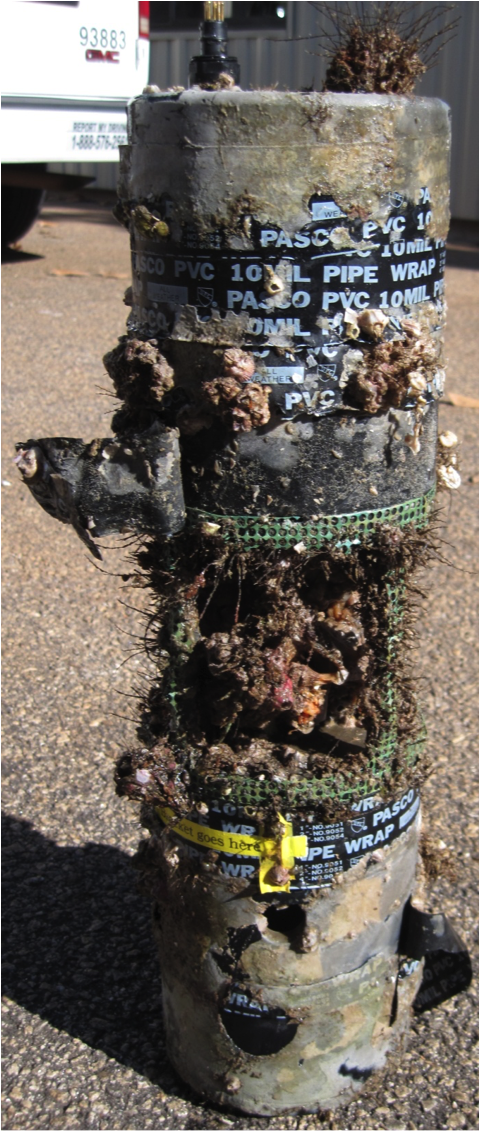
\includegraphics[width=0.9\textwidth]{figs/Foul.png}
}
\end{minipage}
\begin{minipage}[t]{0.5\textwidth}
Please help us speed up your service by properly cleaning your \instType{} before return.  \instType{}s that are returned with excessive biofouling may be subject to additional cleaning and processing charges.\\

\begin{enumerate}
\item Gently remove biological material from the surface of the \instType{}.  Do not use abrasive pads or metal scrapers as these may damage the housing.\\

%\ifiSAMI
%	% If iSAMI don't talk about brass cage and fibers.
%\else
%	\item If there is significant fouling inside the brass cage areas of the instrument, remove the cage and spray a moderate stream of water to remove what will easily come off.  Be careful of the fiber optics and tubing.  The brass cage can be discarded.\\
%\fi

\ifcase \inst
	% If iSAMI don't talk about brass cage and fibers.
\or
	\item If there is significant fouling inside the brass cage areas of the instrument, remove the cage and spray a moderate stream of water to remove what will easily come off.  Be careful of the fiber optics and tubing.  The brass cage can be discarded.\\
\or
	This is an AFT.
\fi

\item After completing the above steps, please allow 24 to 48 hours in a dry area before packing up the instrument. \textbf{Never wrap a wet \instType{} in plastic and return to Sunburst}.
\end{enumerate}

\ifiSAMI
    \vspace*{6.5cm}
\else
    \vspace*{4cm}
\fi

\noindent
To make cleaning easier, 10\,mil PVC corrosion protection tape can be applied to the \instType{} pre-deployment and then removed along with fouling at the end of deployment. This is available from many suppliers such as McMaster Carr:
\newline
\url{http://www.mcmaster.com/#7621A11}
\end{minipage}


\newpage
\restoregeometry

\section{Warnings and Safety}

To prevent damage to the Submersible Autonomous Moored Instrument (\instType{}), please carefully read the operating instructions before attempting to use your instrument. The cable provided is for bench-top programming and download of the \instType{} data, and can be used for shallow laboratory submersion.  IT IS NOT MEANT TO BE DEPLOYED!


\subsection*{Handling}

The \instType{} is reagent-based with the reagent stored in sealed foil bags underneath the instrument.  It is possible, though very unlikely, that these bags may leak or rupture. In case of exposure to the reagent, please refer to the material safety data sheets in the appendix of this manual.


\subsection*{\instType{} Power}

The \instType{} can be powered externally (10--13\,VDC). Observe common safety protocols when using any external power supplies, especially in a wet environment.  While the instrument is diode protected for reverse voltage, large voltages will damage the instrument.  Connect with care!


\section{Introduction to the \instType{}-pH}

\subsection{What's in the box...}

The rugged instrument case for your \instType{} should contain the following upon arrival:

% Use a different list for iSAMI/SAMI
\ifiSAMI
    \begin{enumerate}
    \item \instType{}-pH Instrument.
    \item \instType{} Operating Manual.
    \item Communication/Power Cable.
    \item \instType{} Software Disc.
    \item De-Clogging kit (for air-locked pump).
    \item Pre-Deployment Checklist.
    \item Battery pack (if ordered).
    \end{enumerate}
\else
    \begin{enumerate}
    \item \instType{}-pH Instrument.
    \item \instType{} Operating Manual.
    \item Communication/Power Cable.
    \item \instType{} Software Disc.
    \item De-Clogging kit (for air-locked pump).
    \item Pre-Deployment Checklist.
    \item Any external instruments, extra batteries or reagent ordered, though these may ship separately.
    \item Pre-wetted inlet filter.
    \end{enumerate}
    
    \noindent
    Your stainless steel mooring cage, if ordered for a \instType{}, will ship separately.
\fi

\noindent
If any of these materials is damaged or missing, please contact Sunburst Sensors immediately.


\subsection{Overview of Communication}

\begin{figure}[ht]
\centering
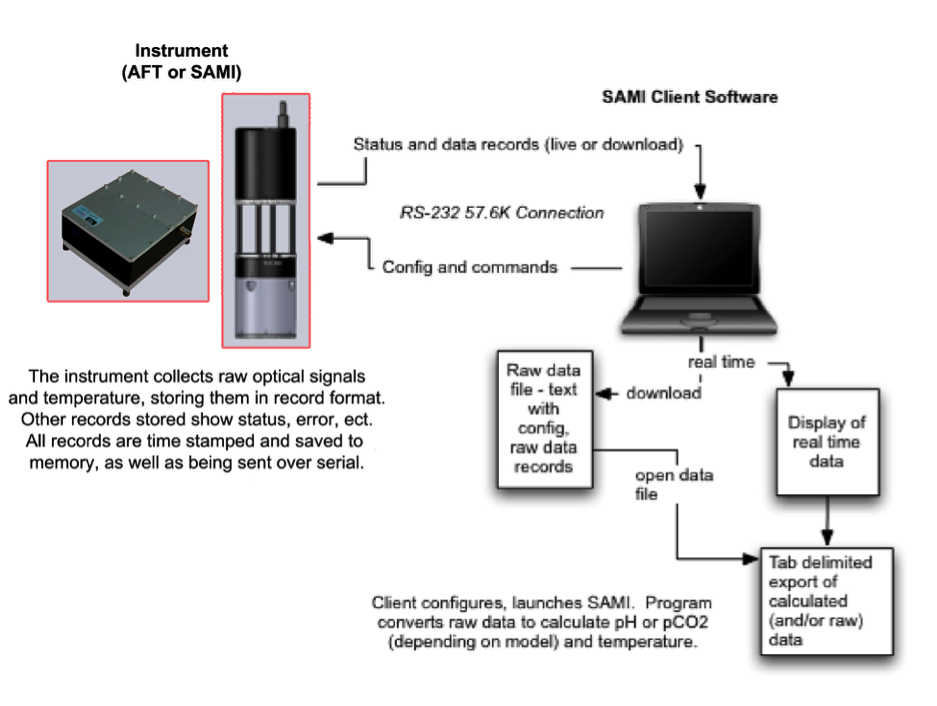
\includegraphics[width=1.0\textwidth]{figs/OperationFig.png}
\caption{Operation overview.}
\label{fig:OperationFig}
\end{figure}

Figure \ref{fig:OperationFig} gives an overview of how the \instType{}-pH operates and interacts with the \textbf{SAMI_Client} software.  The \instType{} uses a time-stamped, records based system to store and transmit data.  There are two main types of records; Data and Status.  Data records consist of raw measurement data, while status records contain information about the state of the instrument (start, stop, battery low, error, etc.)

Once running, all records are stored to internal memory for later download.  Additionally they are transmitted over the serial port, though for energy efficiency the port only wakes up long enough to send the data. 

Data records transmitted to the client can be displayed in real time.

The \textbf{SAMI_Client} software sends configuration data (start time, sampling interval, etc.) and commands to the \instType{} (start, stop, erase, etc.)  It also allows the download of data from the instrument.  Data is downloaded into a text file that contains the configuration data and raw signal intensities as well as any status records.  The user can then open and parse that file using the \textbf{SAMI_Client}.

Data can be exported to tab-delimited files for use in other graphing or analytical software from the data viewer.


\subsection{\instType{}-pH Hardware}

% if SAMI, talk about pressure housing and p/v housing, etc.
\ifiSAMI
    The \instType{} consists of the water sealed electronics housing and the reagent housing.  These are described below.
\else
    The \instType{} consists of a pressure housing, reagent housing, pump/valve housing and the sampling area.  These are described below.
\fi

\ifiSAMI
    \begin{wrapfigure}[25]{r}{0.5\textwidth}
    \centering
       \includegraphics[width=0.9\textwidth]{figs/\instType_pic.png}
    \caption{\instType{}-pH.}
    \label{fig:\instType{}pH}
    \end{wrapfigure}
\else
    \begin{wrapfigure}[32]{r}{0.5\textwidth}
    \centering
       \includegraphics[width=0.9\textwidth]{figs/\instType_pic.png}
    \caption{\instType{}2-pH.}
    \label{fig:\instType{}pH}
    \end{wrapfigure}
\fi


% Use a different list to describe iSAMI/SAMI
\ifiSAMI
    \textbf{Electronics Housing:} The electronics housing contains the controller board, back-up batteries, optics, integrated pump, valve, mixer, and optical cell. \textbf{The \instType{} pump is not pressure-compensated. The \instType{} can therefore only be used from the surface to 3 m depth.} The communication-power bulkhead fitting is located on the top of the housing. The tubing protruding from the top of the \instType{} is the sample outlet.\\
    
    \textbf{Reagent Housing:} The reagent housing, found on the bottom of the instrument, holds and protects the reagent bag but is open to the environment to maintain pressure equilibrium. A bag containing nanopure water or \say{blank} will be attached to the inlet tubing protruding from the reagent housing. This tubing is the sample inlet, and the bag must therefore be removed before deploying the \instType{}. Be careful to not introduce air bubbles when removing the bag.\\
    
    \textbf{Cable:} See Section \ref{Cable}.
\else
    \textbf{Pressure Housing:} The pressure housing contains the controller board, batteries and optics. The communication-power bulkhead fitting is located on the top of the housing. Other bulkhead fittings will be present if external instruments are being supported.\\
    
    \textbf{Sampling Area:} Wrapped in a protective perforated brass housing (not shown), this area is open to the environment. It contains the flow cell, the mixing coil, fiber optics and thermistor. A bag containing nanopure water or \say{blank} will be attached to the inlet tubing protruding from the brass housing. This tubing is the sample inlet, and the bag must therefore be removed before deploying the \instType{}. Be careful to not introduce air bubbles when removing the bag.\\
    
    \textbf{Pump/Valve Housing:} This pressure compensated housing is filled with low viscosity silicon oil to maintain a hydrostatic pressure environment for the pump and valve contained within. A diaphragm on the bottom of the housing makes contact with external pressure. The pump drives reagent through the system, while the valve selects between reagent and seawater.\\
    
    \textbf{Reagent Housing:} The reagent housing, found on the bottom of the instrument, holds and protects the reagent bag but is open to the environment to maintain pressure equilibrium.\\
    
    \textbf{Cable:} See Section \ref{Cable}.
\fi